\chapter{Implementacja}
W tym rozdziale przybliżone zostało działanie aplikacji w odniesieniu do wykorzystywanych technologii.

\section{Stos technologiczny}

Przed przystąpieniem do przeglądu konkretnych rozwiązań i bibliotek, które zostały wykorzystane podczas tworzenia aplikacji. 
\begin{itemize}
    \item Jako platforma programistyczna backendowy został wykorzystany ASP.NET CORE 3.0, w którym można pisać w języku C\#. Nadaje się doskonale do pisania interfejsu programistycznego aplikacji.\cite{asp} Dzięki architekturze MVC można było w sposób zrozumiały i ścisły sposób opisać reguły w jaki programy komunikują się ze sobą.\cite{asp} W skrócie nazywa się to API. Jest ono definiowane już na poziomie kodu źródłowego, a jego zadaniem jest przekazanie wyszczególnionego spisu struktur danych, podprogramów, klas oraz protokołów do komunikacji.\cite{api} Funkcje API są użyczane jako zasób w sieci.
    \item Jako platforma programistyczna frontendowa został wykorzystany Angular w wersji 8.0.0. Został on napisany w języku TypeScript, który jest nadzbiorem języka JavaScript, który został poszerzony o funkcje typowania oraz dopełniające struktury językowe niedostępne w ECMAScript.\cite{ts} ECMAScript jest znormalizowaną specyfikacją skryptowego języka programowania, której implementacją jest między innymi JavaScript. Angular jest otwarty i pozwala na tworzenie SPA, czyli aplikacji jednostronicowej. Jest to aplikacja lub witryna internetowa, która ma możliwość wchodzenia w interakcję z użytkownikiem poprzez dynamiczne przepisywanie bieżącej strony zamiast ładowania całych nowych stron z serwera. Podejście takie pozwala unikać zakłóceń w obsłudze między kolejnymi stronami, dzięki czemu zachowanie programu jest bliższe do okienkowej aplikacji komputerowej. W SPA cały niezbędny kod, czyli HTML, JavaScript i CSS są pobierane przy pojedynczym przeładowaniu strony lub potrzebne zasoby są dynamicznie ładowane, a później dodawane do strony w razie konieczności(zazwyczaj w odpowiedzi na działania użytkownika).\cite{spa}
    \item Jako baza danych wykorzystywany jest PostgreSQL. Jest otwartym systemem zarządzania relacyjnymi bazami danych (DBMS), który został stworzony przez ogólnoświatowy zespół ochotników. Dzięki czemu nie jest kontrolowany przez żadną korporację czy inny podmiot prywatny, a kod źródłowy jest dostępny za darmo dla każdego. PostgreSQL obsługuje między innymi transakcje, podselekcje, wyzwalacze, integralność referencyjną kluczy obcych, widoki.\cite{postgresql}
\end{itemize}
Poniżej opisano wykorzystane narzędzia:
\begin{itemize}
    \item Rider -- zintegrowane środowisko programistyczne, czyli program który udostępnia złożoną funkcjonalność obejmującą tworzenie oprogramowania, przede wszystkim edycję kodu źródłowego oraz jego kompilację. Ponadto umożliwia debugowanie aplikacji oraz integruje się z wykorzystywaną bazą danych. Zostało wydane oraz jest rozwijane przez firmę JetBrains. Środowisko to pozwala na tworzenie różnorakich aplikacji w .NET oraz obsługuję również frameworki frontendowe takie jak Angular oraz React.\cite{rider} Umożliwia również używanie wygodnych skrótów klawiszowych, które w znaczący sposób przyśpieszają pracę nad oprogramowaniem.
    \item TSLint -- jest rozszerzalnym narzędziem do statycznej analizy kodu napisanego w TypeScript pod kątem czytelności, łatwości utrzymania oraz błędów funkcjonalnych. Można go dostosowywać do własnych reguł, konfiguracji i formatów.\cite{tslint}
    \item Git -- jest otwarto-źródłowym rozproszonym systemem kontroli wersji, które służy do monitorowania zmaina w kodzie źródłowym w trakcie tworzenia oprogramowania. Przeznaczony on jest do koordynowania pracy programistów, ale może również służyć do śledzenia dowolnych plików. Git charakteryzuje się szybkością, integralność danych oraz obsługa rozproszonych, nieliniowych przepływów pracy. Został stworzony przez Linusa Torvaldsa w 2005 roku w celu rozwoju jądra Linuksa. Podobnie jak w innych rozproszonych systemach kontroli wersji i w przeciwieństwie do systemów klient-serwer, każdy katalog Git na odrębnych komputerach jest pełnoprawnym repozytorium z zachowaniem pełnej historii i pełnych możliwości śledzenia wersji, niezależnie od dostępu do serwera centralnego.\cite{git}.
\end{itemize}

\section{API}
Zgodnie z architekturą zaprezentowaną w Rozdziale \ref{chap:arch_log} oraz Rozdziale \ref{chap:arch_fiz} API zostało zaimplementowana w następujący sposób.
\subsection{Struktura}
Na Rysunku \ref{fig:struct_api} przedstawiono strukturę backendu, który pełni funkcję interfejsu programistycznego aplikacji.
\begin{figure}[H]
\centering
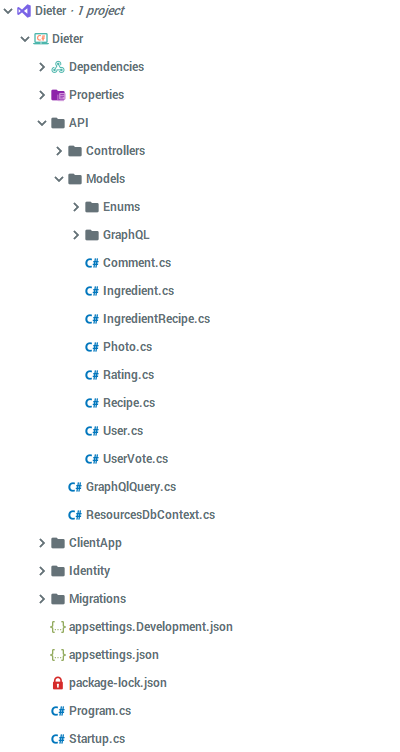
\includegraphics[width=.5\textwidth]{rys/struktura-api.png}
\caption{Struktura API}
\label{fig:struct_api}
\end{figure}

\subsection{Model danych i integracja z bazą danych}
Na początku zostały zdefiniowane modele danych, które później za pomocą biblioteki Entity Framework Core zostały zmapowane do relacyjnej bazy danych. Poniżej przedstawiono przykładowy model.
\begin{lstlisting}[language={[Sharp]C}]
 public class Recipe
    {
        
        public int RecipeId { get; set; }
        public virtual User Author { get; set; }
        public string Name { get; set; }
        public string Description { get; set; }
        public int? Calories { get; set; }
        public int? Weight { get; set; }
        public int? EstTime { get; set; }
        public Difficulty? Difficulty { get; set; }
        public virtual Rating Rating { get; set; }
        
        public virtual ICollection<Comment>
        Comments { get; set; }
        public virtual ICollection<IngredientRecipe>
        IngredientRecipes { get; set; }
    }
\end{lstlisting}
Obiekty domyślnie są mapowane na atrybuty, które mogą zawierać wartość zerową. Typy prymitywne takie jak na przykład \texttt{int} nie posiadają tej właściwości, więc aby w bazie danych mogły być wartością opcjonalną należy dodać znak pytajnika po typie. Modyfikator \texttt{virtual} pozwala na leniwe załadowanie danych, dzięki czemu później wykonując kweredndy GraphQL będzie możliwe swobodne poruszanie się między tabelami. Na podstawie powyższego kodu powstała tabela przedstawiona na Rysunku \ref{fig:recipe_table}. Jak widać oprócz atrybutów zostały utworzone klucze obce do innych tabel.

\begin{figure}[H]
\centering
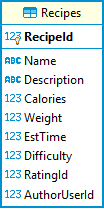
\includegraphics[width=.2\textwidth]{rys/recipe.png}
\caption{Tabela przepisu}
\label{fig:recipe_table}
\end{figure}

Po utworzeniu wszystkich modelów zostały one użyte do zainicjalizowania kontekstu bazy danych, który po połączeniu z bazą danych pozwala na łatwą manipulację danych. Poniżej przedstawiono tworzenie takiego kontekstu.

\begin{lstlisting}[language={[Sharp]C}]
  public ResourcesDbContext(DbContextOptions
  <ResourcesDbContext> options) : base(options)
        {
        }
        protected override void OnModelCreating
        (ModelBuilder modelBuilder)
        {
            modelBuilder.Entity<IngredientRecipe>()
            .HasKey(ir => new {ir.IngredientId, ir.RecipeId});
        }
        
        protected override void OnConfiguring
        (DbContextOptionsBuilder optionsBuilder)
        {
            optionsBuilder.UseLazyLoadingProxies();
        }

        public DbSet<Comment> Comments { get; set; }
        public DbSet<Ingredient> Ingredients { get; set; }
        public DbSet<Rating> Ratings { get; set; }
        public DbSet<Recipe> Recipes { get; set; }
        public DbSet<User> Users { get; set; }
        public DbSet<IngredientRecipe> IngredientRecipes 
        { get; set; }
        public DbSet<UserVote> UserVotes { get; set; }
    }
\end{lstlisting}

Jak widać podano w nim wszystkie utworzone wcześniej modele. Bardzo ciekawym rozwiązaniem jest użycie metody \texttt{r.UseLazyLoadingProxies ( )}, która umożliwia leniwe ładowanie, dzięki czemu można odwoływać się coraz głębiej w obiekty. Znacząco ułatwia to późniejszą pracę. Dodatkowo powiązano ze sobą klucze składniku \texttt{IngredientId} oraz przepisu \texttt{RecipeId} w modelu pośredniczącym \texttt{IngredientRecipe}. Działanie to powoduje stworzenie relacji wiele do wielu, która po wysłaniu struktury do bazy danych będzie w postaci dodatkowej tabeli.\newline

Połączenie z bazą danych było bardzo proste. Wystarczyło wywołać poniższą funkcję oraz zdefiniować w osobnym pliku dane potrzebne do połączenia z bazą danych.
\begin{lstlisting}[language={[Sharp]C}]
 services.AddDbContext<ResourcesDbContext>(opt =>
                opt.UseNpgsql(Configuration
                .GetConnectionString("DefaultConnection")));
\end{lstlisting}
Poniżej znajdują się przykładowe dane potrzebne do połączenia z serwerem PostgreSQL.
\begin{lstlisting}
  "ConnectionStrings": {
    "DefaultConnection": "User ID =postgres;Password=pass;
    Server=localhost;Port=5432;Database=DieterDb;
    Integrated Security=true;Pooling=true;",
  },
\end{lstlisting}

Oprócz modeli danych zostały też stworzone wyliczeniowe typy danych, które są później wykorzystywane w owych modelach. Przykładowy typ wyliczeniowy został przedstawiony poniżej.

\begin{lstlisting}[language={[Sharp]C}]
 public enum Difficulty
    {
        VeryEasy,
        Easy,
        Medium,
        Hard,
        VeryHard,
    }
\end{lstlisting}

\subsection{Kontroler}
Kontroler w API służy do obsługi przychodzących żądań HTTP i odsyła odpowiedź. W aplikacji w sytuacji korzystania ze standardu REST lub SOAP w zdecydowanej większości wypadków będzie występował więcej niż jeden kontroler. Ale ze względu na wykorzystanie w projekcie GraphQL występuje tylko jeden kontroler. Tak wynika ze specyfikacji tego standardu.\cite{gqlcode} Na poniższym listingu znajduje się ten kontroler.
\begin{lstlisting}[language={[Sharp]C}]
[Route("graphql")]
public class GraphQlController : Controller
    {
        private readonly ResourcesDbContext _db;
        private readonly UserManager<AppUser> _userManager;
        private readonly SignInManager<AppUser> _signInManager;

        public GraphQlController(ResourcesDbContext db,
            UserManager<AppUser> userManager,
            SignInManager<AppUser> signInManager)
        {
            _db = db;
            _userManager = userManager;
            _signInManager = signInManager;
        }

        public async Task<IActionResult> 
        Post([FromBody] GraphQlQuery query)
        {
            var inputs = query.Variables.ToInputs();

            var schema = new Schema()
            {
                Query = new DieterQuery(_db),
                Mutation = new DieterMutation
                (_db, _userManager, _signInManager)
            };

            var result = await new DocumentExecuter()
            .ExecuteAsync(_ =>
            {
                _.Schema = schema;
                _.Query = query.Query;
                _.OperationName = query.OperationName;
                _.Inputs = inputs;
            }).ConfigureAwait(false);

            if (result.Errors?.Count > 0)
            {
                return BadRequest();
            }

            return Ok(result);
        }
    }
\end{lstlisting}

Jak widać tworzy schemat na podstawie typów, kwerend oraz mutacji. Następnie zwraca wynik o wcześniej zdefiniowanej strukturze. W razie potrzeby kontroler może zwrócić też błąd. Na samym początku podana jest trasa do połączenia się z danym punktem końcowym, będzie ona potrzebna później w aplikacji klienckiej. 

\subsection{GraphQL}
Na Rysunku \ref{fig:graphql_table} przedstawiono strukturę plików wykorzystaną w projekcie aplikacji.
Dzielą się one na pliki definiujące:
\begin{itemize}
    \item typy, które są tworzone na podstawie modeli oraz typów wyliczeniowych,
    \item typy wejściowe, które są przekazywane jako argumenty do mutacji i kwerend,
    \item kwerendy, które służą do pobierania danych, zawierają w sobie pobieranie danych z serwera, obliczenia i działania na nich oraz mapowanie na odpowiednie typy,
    \item mutacje, które są operacjami modyfikującymi stan danych, czyli edycja, dodawanie oraz usuwanie. Muszą zwrócić jakiś typ tak samo jak kwerenda.
\end{itemize}
Razem tworzą schemat GraphQL, który można traktować jako kontrakt między backendem, a frontendem. Jego wcześniejsze zdefiniowanie pozwala w większych zespołach na bardziej niezależną od siebie pracę. W jednoosobowym projekcie nie ma to aż tak wielkiego znaczenia.

\begin{figure}[H]
\centering
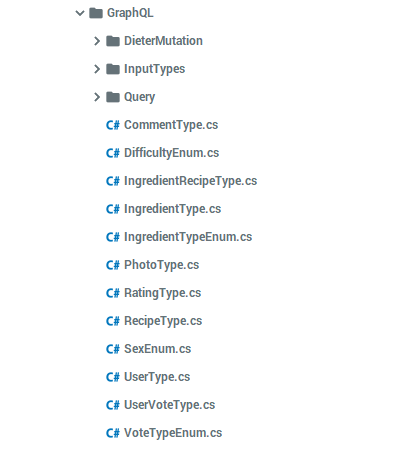
\includegraphics[width=.7\textwidth]{rys/struktura-graphql.png}
\caption{Struktura plików GraphQL}
\label{fig:graphql_table}
\end{figure}

Poniżej znajduje się przykładowa kwerenda GraphQL, która zwraca wszystkie komentarze dla przepisu o podanym jako argument numerze identyfikującym. Dzięki wykorzystaniu Entity Framework Core i języka LINQ, wykonywane jest filtrowanie danych na tabeli \textit{Comments}, szukając rekordów o podanym wcześniej numerze przepisu. Zwrócony typ jest automatycznie mapowany na typ GraohQL.
\begin{lstlisting}[language={[Sharp]C}]
 Field<ListGraphType<CommentType>>(
      "getComments",
       arguments: new QueryArguments(
          new QueryArgument<IdGraphType> {Name = "recipeId"}),
       resolve: context =>
         {
          var recipeId = context.GetArgument<int?>("recipeId");
          return db.Comments
          .Where(x => x.Recipe.RecipeId == recipeId);
      });
\end{lstlisting}

Natomiast na poniższym listingu przedstawiono przykładową mutację. Zostało tu pokazane dodawanie komentarza. Jako argumenty przekazywane są treść komentarza oraz numery identyfikacyjne autora i przepisu, do którego komentarz jest wystawiany. Znowu dzięki użyciu Entity Framework Core w prosty sposób można było wykonać operację na bazie danych. Po edycji obiektu w kodzie, który ma swoje odzwierciedlenie w strukturze bazy danych i wywołaniu metody \texttt{SaveChanges()} na kontekście bazy danych, baza danych zostaje zaktualizowana o przeprowadzone zmiany.

\begin{lstlisting}[language={[Sharp]C}]
Field<CommentType>(
    "addComment",
    arguments: new QueryArguments(
        new QueryArgument<NonNullGraphType
        <AddCommentInputType>> {Name = "comment"},
        new QueryArgument<NonNullGraphType
        <IdGraphType>> {Name = "authorUserId"},
        new QueryArgument<NonNullGraphType
        <IdGraphType>> {Name = "recipeId"}),
    resolve: context =>
    {
        var comment = context.GetArgument<Comment>("comment");
        var authorUserId = context.GetArgument<int>("authorUserId");
        var recipeId = context.GetArgument<int>("recipeId");

        //add rating record
        var rating = new Rating();
        db.Ratings.Add(rating);
        db.SaveChanges();
        comment.Rating = rating;

        //add author
        comment.Author = db.Users
        .FirstOrDefault(x => x.UserId == authorUserId);
        //add recipe
        comment.Recipe = db.Recipes
        .FirstOrDefault(x => x.RecipeId == recipeId);

        //add comment
        comment.PublicationDate = DateTime.Now;
        db.Comments.Add(comment);
        db.SaveChanges();

        return comment;
    });
\end{lstlisting}

\subsection{Identity Core}
Jest to system, który obsługuje funkcje rejestracji oraz logowania użytkownik oraz uwierzytelnianie i autoryzację. Użytkownicy mogą stworzyć konto z danymi, które są zapisywane w odpowiednich tabelach wcześniej wygenerowanej bazy danych lub skorzystać z danych logowania zewnętrznego dostawcy takiego jak na przykład Facebook, Google, Microsoft, Twitter. Jej strukturę przedstawiono na Rysunku \ref{fig:identity_schema}. Przechowywanie tożsamości domyślnie jest skonfigurowane do wykorzystywania SQL Server, ale z powodzeniem można używać innych systemów obsługi baz danych. W aplikacji wykorzystano integrację z PostgreSQL. Implementacja została wykonana dzięki wbudowanej w .NET Core możliwości integracji z aplikacją. Wystarczyło dodanie biblioteki przez menedżer pakietów NuGet oraz krótka konfiguracja.


\begin{figure}[H]
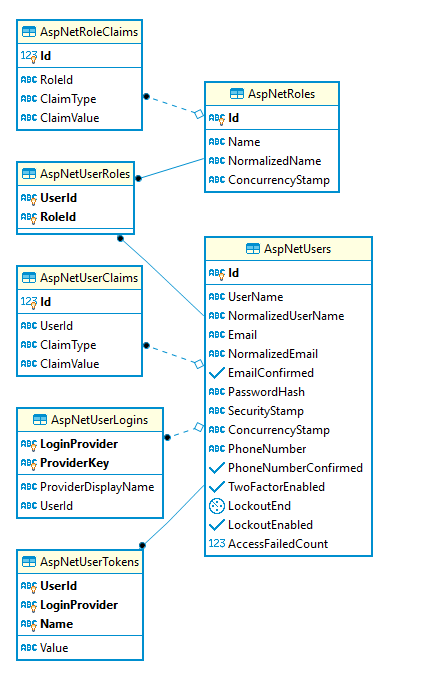
\includegraphics[width=.9\textwidth]{rys/identity-baza.png}
\caption{Schemat bazy danych tożsamości}
\label{fig:identity_schema}
\end{figure}

\section{Aplikacja przeglądarkowa}
Aplikacja przeglądarkowa została napisana z pomocą frameworku Angular i skojarzonych z nim bibliotek. W poniższym rozdziale została opisana jej implementacja. Za Rysunku \ref{fig:front_schem} została przedstawiona struktura projektu.


\begin{figure}[H]
\centering
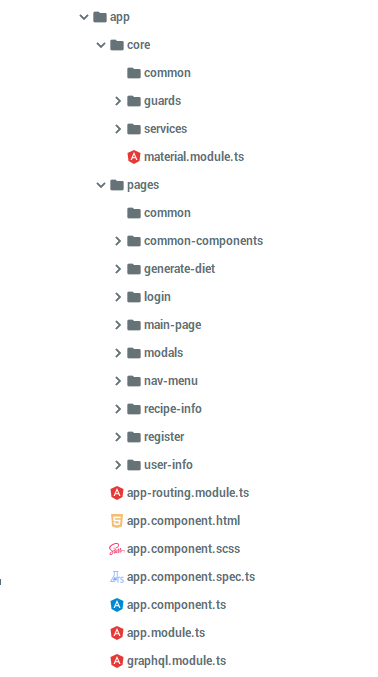
\includegraphics[width=.7\textwidth]{rys/front-schem.png}
\caption{Struktura plików aplikacji przeglądarkowej}
\label{fig:front_schem}
\end{figure}

\subsection{Połączenie z API}
Do połączenia został wykorzystany klient Apollo. Jest to niezwykle elastyczny, oparty na pracy zaangażowanej społeczności klient GraphQL dla platformy Angular.\cite{apollo} Został zaprojektowany, aby ułatwić tworzenie komponentów interfejsu użytkownika, które pobierają dane za pomocą GraphQL. Rozwiązanie to zostało wybrane ponieważ:
\begin{itemize}
    \item przystosowalność -- można wykorzystać go w istniejącej aplikacji,
    \item uniwersalność -- jest kompatybilny z dowolną konfiguracją, dowolnym serwerem lub schematem GraphQL,
    \item nieskomplikowanie -- w łatwy sposób można pobrać dane, a wykorzystaniem dodatkowej, bardziej zaawansowanej funkcjonalności zostawić sobie na później,
    \item zrozumiały i łatwy do sprawdzania,
    \item mały i elastycznym -- nie potrzebuje wielu zasobów do poprawnego działania, a jego rdzeń został skompresowany do rozmiaru poniżej 12 KB,
    \item otwarto-źródłowy -- rozbudowana społeczność trwa o rozwój biblioteki.
\end{itemize}


W poniższym kodzie przedstawiono sposób łączenia się z API. W stałej \texttt{uri} przechowywany jest endpoint backendu. Następnie tworzone jest połączenie poprzez użycie funkcji \texttt{create()} w obiekcie \texttt{httpLink}.
\begin{lstlisting}[language=JavaScript]
const uri = 'https://localhost:5001/graphql';
export function createApollo(httpLink: HttpLink) {
  return {
    link: httpLink.create({uri}),
    cache: new InMemoryCache(),
  };
}

@NgModule({
  exports: [ApolloModule, HttpLinkModule],
  providers: [
    {
      provide: APOLLO_OPTIONS,
      useFactory: createApollo,
      deps: [HttpLink],
    },
  ],
})
export class GraphQLModule {}
\end{lstlisting}

\subsection{Pobieranie danych}
Pobieranie danych w prosty i przewidywalny sposób jest jedną z podstawowych funkcji klienta Apollo.
Na początku należało napisać kwerendę w języku GraphQL. Przykładowa została przedstawiona poniżej. Została tu przedstawiona jedna z ważniejszych zalet GraphQL, a mianowicie możliwość odwoływania się ,,w głąb'' typów danych. Na przykład z poziomu przepisu możemy uzyskać informacje o autorze.
\begin{lstlisting}
query getRecipe($recipeId: ID){
  getRecipe(recipeId: $recipeId){
    recipeId
    description
    calories
    difficulty
    estTime
    weight
    author{
      userName
      userId
    }
    rating{
      downVotes
      upVotes
    }
  }
}
\end{lstlisting}
Następnie na podstawie schematu GraphQL i wcześniej napisanej kwerendy należało wygenerować odpowiednie typy i funkcje zrozumiałe przez język TypeScript. Posłużyło do tego narzędzie graphql-codegen, które na podstawie pliku \texttt{schema.graphql} tworzy wymagane do dalszego działania pliki.\\
Kolejnym krokiem było skorzystanie z mechanizmu wstrzykiwania zależności, czyli dodanie w konstruktorze komponentu obiektu, który z wcześniej wygenerowanych danych jest w stanie komunikować się z API. Przykładowy konstruktor został pokazany poniżej.
\begin{lstlisting}[language=JavaScript]
  constructor(private route: ActivatedRoute,
              private getRecipeGQL: GetRecipeGQL,
              private commonTypes: CommonTypesService,
              private snackBar: MatSnackBar,
              private userService: UserService,
              private voteGQL: VoteGQL,
              private router: Router,
              public dialog: MatDialog) {
  }
\end{lstlisting}
Obiekty z sufiksem \texttt{GQL} odpowiadają za wykonywanie kwerend lub mutacji.\\
Następnym krokiem było pobranie danych, co zostało zobrazowane w poniższej metodzie.
\begin{lstlisting}[language=JavaScript]
  private getRecipe(recipeId: string) {
    this.subscription.add(this.getRecipeGQL
      .fetch({recipeId})
      .subscribe(result => {
        this.loading = result.loading;
        this.recipe = result.data.getRecipe;
      }));
  }
  \end{lstlisting}
  Do zmiennej \texttt{loading} zapisywany jest stan ładowania. Jest on konieczny do wizualizacji procesu pobierania danych. A wszystkie dane dotyczące przepisu przekazywane są do zmiennej \texttt{recipe}, z której później można się bezpośrednio odwoływać w szablonie.
  \subsection{Modyfikacja dancyh}
  Odbywa się w bardzo podobny sposób, co pobieranie danych, schemat praktycznie jest ten sam. Na początku należy napisać mutację, należ